% !TeX root = main.tex

\hypertarget{linear-functions}{%
\section{Linear Functions}\label{linear-functions}}

\hypertarget{cost-revenue-and-profit}{%
\subsection{Cost, Revenue and Profit}\label{cost-revenue-and-profit}}

A company has fixed costs of \$10,000 for equipment and variable costs
of \$15 for each unit of output. The sale price for each unit is \$25.
What is total cost, total revenue and total profit at varying levels of
output?

\hypertarget{the-slope-intercept-form-equation}{%
\subsection{The Slope-Intercept Form
Equation}\label{the-slope-intercept-form-equation}}

The slope of a line measures the steepness, in other words, ``rise''
over ``run'', or rate of change of the line. Using the rectangular
coordinate system, the \textbf{\emph{slope}} \(m\) of a line is defined
as \[
m=\dfrac{y_2-y_1}{x_2-x_1}=\dfrac{\text{rise}}{\text{run}}=\dfrac{\text{change in the output }y}{\text{change in the input } x},
\] where \((x_1, y_1)\) and \((x_2, y_2)\) are any two distinct points
on the line. If the line intersects the \(y\)-axis at the point
\((0, b)\), then a point \((x, y)\) is on the line if and only if \[
y=mx+b.
\] This equation is called the \textbf{\emph{slope-intercept form}} of
the line.

\hypertarget{point-slope-form-equation-of-a-line}{%
\subsection{Point-Slope Form Equation of a
Line}\label{point-slope-form-equation-of-a-line}}

Suppose a line passing through the point \((x_0, y_0)\) has the slope
\(m\). Solving from the slope formula, we see that any point \((x, y)\)
on the line satisfies the equation equation \[
y=m(x-x_0)+y_0
\] which is called the \textbf{\emph{point-slope form}} equation.

\hypertarget{linear-function}{%
\subsection{Linear Function}\label{linear-function}}

A \textbf{\emph{linear function}} \(f\) is a function whose graph is a
line. An equation for \(f\) can be written as \[f(x) = mx + b\] where
\(m\) is the slope and \(b=f(0)\).

A function \(f\) is a linear function if the following equalities hold
\[
\dfrac{f(x_2)-f(x_1)}{x_2-x_1}
=\dfrac{f(x_3)-f(x_1)}{x_3-x_1}
\] for any three distinct points \((x_1, y_1)\), \((x_2, y_2)\) and
\((x_3, y_3)\) on the graph of \(f\).

\hypertarget{equations-of-linear-functions}{%
\subsection{Equations of Linear
Functions}\label{equations-of-linear-functions}}

\begin{example}

Find the slope-intercept form equation for the linear function \(f\)
such that \(f(2)=5\) and \(f(-1) = 2\).

\end{example}
\vspace*{6\baselineskip}

\hypertarget{graph-a-linear-function-by-plotting-points}{%
\subsection{Graph a Linear Function by Plotting
Points}\label{graph-a-linear-function-by-plotting-points}}

\begin{example}

Sketch the graph of the linear function \(f(x)=-\frac12 x + 1\).

\end{example}
\vspace*{6\baselineskip}

\hypertarget{horizontal-and-vertical-lines}{%
\subsection{Horizontal and Vertical
Lines}\label{horizontal-and-vertical-lines}}

A \textbf{\emph{horizontal line}} is defined by an equation \(y=b\). The
slope of a horizontal line is simply zero. A \textbf{\emph{vertical
line}} is defined by an equation \(x=a\). The slope of a vertical line
is \textbf{undefined}.

A vertical line gives an example that a graph is not a function of
\(x\). Indeed, the vertical line test fails for a vertical line.

\hypertarget{explicit-function}{%
\subsection{Explicit Function}\label{explicit-function}}

When studying functions, we prefer a clearly expressed function rule.
For example, in \(f(x)=-\frac23x+1\), the expression \(-\frac23x+1\)
clearly tells us how to produce outputs. For a function \(f\) defined by
an equation, for instance, \(2x+3y=3\), to find the function rule (that
is an expression), we simply solve the given equation for \(y\). \[
\begin{aligned}
2x+3y&=3\\
3y&=-2x+3\\
y&=-\frac23x+1.
\end{aligned}
\] Now, we get \(f(x)=-\frac23x+1\).

\hypertarget{perpendicular-and-parallel-lines}{%
\subsection{Perpendicular and Parallel
Lines}\label{perpendicular-and-parallel-lines}}

Any two vertical lines are parallel. Two non-vertical lines are
\textbf{\emph{parallel}} if and only if they \textbf{have the same
slope}.

A line that is parallel to the line \(y=mx+a\) has an equation
\(y=mx+b\), where \(a\neq b\).

Horizontal lines are perpendicular to vertical lines. Two non-vertical
lines are \textbf{\emph{perpendicular}} if and only if \textbf{the
product of their slopes is \(-1\)}.

A line that is perpendicular to the line \(y=mx+a\) has an equation
\(y=-\frac1m x+b\).

\hypertarget{finding-equations-for-perpendicular-or-parallel-lines}{%
\subsection{Finding Equations for Perpendicular or Parallel
Lines}\label{finding-equations-for-perpendicular-or-parallel-lines}}

\begin{example}

Find an equation of the line that is parallel to the line \(4x+2y=1\)
and passes through the point \((-3, 1)\).

\end{example}
\vspace*{6\baselineskip}

\begin{example}

Find an equation of the line that is perpendicular to the line
\(4x-2y=1\) and passes through the point \((-2,3)\).

\end{example}
\vspace*{6\baselineskip}

\subsection{Practice}

\begin{exercise}

Find the slope of the line passing through

\begin{enumerate}
\item
  \((3,5)\) and \((-1, 1)\)
\item
  \((-2,4)\) and \((5, -2)\).
\end{enumerate}

\end{exercise}
\vspace*{2\baselineskip}

\begin{exercise}

Find the point-slope form equation of the line with slope \(5\) that
passes though \((-2, 1)\).

\end{exercise}
\vspace*{6\baselineskip}
\begin{exercise}

Find the point-slope form equation of the line passing thought
\((3, -2)\) and \((1,4)\).

\end{exercise}
\vspace*{6\baselineskip}
\begin{exercise}

Find the slope-intercept form equation of the line passing through
\((6, 3)\) and \((2, 5)\).

\end{exercise}
\vspace*{6\baselineskip}
\begin{exercise}

Determine whether the linear functions \(f(x)\) and \(h(x)\) with the
following values \(f(-2)=-4\) \(f(0)=h(0)=2\) and \(h(2)=8\) define the
same function. Explain your answer.

\end{exercise}
\vspace*{6\baselineskip}
\begin{exercise}

Suppose the points \((5, -1)\) and \((2, 5)\) are on the graph of a
linear function \(f\). Find \(f(-3)\).

\end{exercise}
\vspace*{6\baselineskip}
\begin{exercise}

Graph the functions.

\begin{enumerate}
\item
  \(f(x)=-x + 1\)
\item
  \(f(x)=\frac{1}{2}x - 1\)
\end{enumerate}

\end{exercise}
\vspace*{2\baselineskip}

\begin{exercise}

A storage rental company charges a base fee of \$15 and \$\(x\) per day
for a small cube. Suppose the cost is \$20 dollars for 10 days.

\begin{enumerate}
\item
  Write the cost \(y\) (in dollars) as a linear function of the number
  of days \(x\).
\item
  How much would it cost to rent a small cube for a whole summer (June,
  July and August)?
\end{enumerate}

\end{exercise}
\vspace*{2\baselineskip}

\begin{exercise}

Find an equation for each of the following two lines which pass through
the same point \((-1, 2)\).

\begin{enumerate}
\item
  The vertical line.
\item
  The horizontal line.
\end{enumerate}

\end{exercise}
\vspace*{2\baselineskip}

\begin{exercise}

Line \(L\) is defined by the equation \(2x-5y=-3\). What is the slope
\(m_\parallel\) of the line that is parallel to the line \(L\)? What is
the slope \(m_\perp\) of the line that is perpendicular to the line
\(L\).

\end{exercise}
\vspace*{6\baselineskip}

\begin{exercise}

Line \(L_1\) is defined by \(3y+5x=7\). Line \(L_2\) passes through
\((-1, -3)\) and \((4, -8)\). Determine whether \(L_1\) and \(L_2\) are
parallel, perpendicular or neither.

\end{exercise}
\vspace*{6\baselineskip}

\begin{exercise}

Find the point-slope form and then the slope-intercept form equations of
the line parallel to \(3x-y=4\) and passing through the point
\((2,-3)\).

\end{exercise}
\vspace*{6\baselineskip}

\begin{exercise}

Find the slope-intercept form equation of the line that is perpendicular
to \(4y-2x+3=0\) and passing through the point \((2, -5)\)

\end{exercise}
\vspace*{6\baselineskip}

\begin{exercise}

The line \(L_1\) is defined \(Ax+By=3\). The line \(L_2\) is defined by
the equation \(Ax+By=2\). The line \(L_3\) is defined by \(Bx-Ay=1\).
Determine whether \(L_1\), \(L_2\) and \(L_3\) are parallel or
perpendicular to each other.

\end{exercise}
\vspace*{6\baselineskip}

\begin{exercise}

Use the graph of the line \(L\) to answer the questions.

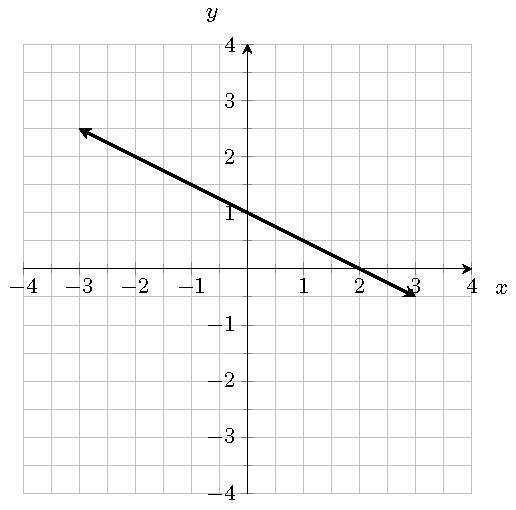
\includegraphics[scale=1]{figs/tikz-perp-prll-exercise.png}

\begin{enumerate}
\item
  Find an equation for the line \(L\).
\item
  Find an equation for the line \(L_\perp\) perpendicular to \(L\) and
  passing through \((1,1)\).
\item
  Find an equation for the line \(L_\parallel\) parallel to \(L\) and
  passing through \((-2,-1)\).
\end{enumerate}



\end{exercise}
\vspace*{2\baselineskip}

\begin{exercise}

Determine whether the points \((-3,1)\), \((-2,6)\), \((3,5)\) and
\((2, 0)\) form a square. Please explain your conclusion.

\end{exercise}

